\documentclass[a4paper,12pt]{article}
\usepackage[margin=2.5cm]{geometry}
\usepackage{authblk}
\usepackage{amsmath,amssymb,graphicx,hyperref,bm,bbm}
\usepackage{tikz}
\usepackage{float}
\usetikzlibrary{decorations.pathmorphing,decorations.markings}

\newcommand{\vev}[1]{\langle #1 \rangle}
\newcommand{\abs}[1]{|#1|}
\newcommand{\order}[1]{\mathcal{O}(#1)}

\begin{document}

\title{Topological soliton coherence scale:\\
  one parameter across seven physical domains}

\author{Jesse C.P. Ting}
\affil{Independent Researcher}



\begin{abstract}
We develop the hypothesis that fundamental fermions are topological
solitons of a compact phase field $\Theta\in[0,2\pi)$, possessing a
single coherence scale $a$ fixed by topology and energy finiteness.
This one parameter produces calculable, falsifiable corrections across
seven independent physical domains: (i)~the electron anomalous magnetic
moment $g{-}2$, (ii)~the hydrogen Lamb shift, (iii)~the $1S$--$2S$
transition frequency, (iv)~Lorentz symmetry emergence, (v)~galactic
dark matter rotation curves via critical slowing of the phase memory
field, (vi)~quantum decoherence and the Born rule, and (vii)~the
selection of gauge rank $r=3$ from soliton moduli counting.  A
three-tier atomic constraint ladder pins $a\leq 0.003$~fm
($\Lambda_{\rm core}\sim 73$~GeV), coincident with the electroweak
scale.  The dark matter mechanism bridges 41~orders of magnitude from
the microscopic anchor $\tau_0 = a/c$ to galactic dynamical times via
Kosterlitz--Thouless critical slowing, with no new free parameters.
We derive a forward prediction $|\delta(g/2)|\sim 4.4\times 10^{-16}$
testable by future precision experiments, and an interferometric
visibility function $V(a,T)$ with a distinctive linear-plus-Gaussian
decay signature distinguishable from standard decoherence models.
The gravitational coupling emerges as the linearized susceptibility
of the background action, not an independent parameter.  Throughout,
$a$ is constrained by data, never fitted.
\end{abstract}

\maketitle

\noindent\textbf{Keywords:} topological soliton, electron form factor, coherence scale, precision atomic spectroscopy, dark matter rotation curves, falsifiable predictions



%======================================================================
\section{Introduction}
\label{sec:intro}
%======================================================================

The electron is the most precisely characterized particle in physics.
Its anomalous magnetic moment is known to sub-part-per-trillion
accuracy~\cite{Fan2023,Morel2020}, the hydrogen $1S$--$2S$ transition
frequency to $4.2\times 10^{-15}$ relative precision~\cite{Parthey2011},
and the classic $2S$--$2P$ Lamb shift to $\sim 2$~kHz~\cite{Bezginov2019}.
These measurements probe quantum electrodynamics at its most stringent
and constrain new physics below the electroweak scale.

In this work we develop a minimal hypothesis: the electron is a
topological soliton of a compact phase field $\Theta\in[0,2\pi)$,
possessing a single coherence scale $a$.  This hypothesis is motivated
by the Energy String Field Theory (ESFT) framework~\cite{ESFT}, in
which the fundamental entity is the phase gradient field
$\varphi\equiv\nabla\Theta$ and particles are topologically stable
solitonic modes.  However, the present derivations rest on only three
ingredients:
\begin{enumerate}
  \item \textbf{Compactness}: $\Theta$ is $S^1$-valued, admitting
    integer winding numbers.
  \item \textbf{Energy finiteness}: The total field energy
    $E[\Theta]=\int d^3x\,|\nabla\Theta|^2$ is finite, forcing
    the soliton profile to regularize below a core scale~$a$.
  \item \textbf{Universality}: Any finite-size structure modifies the
    electromagnetic vertex at leading order as
    $F(q^2)=1-q^2a^2/6+\order{q^4a^4}$, with $a^2\equiv\vev{r^2}$.
\end{enumerate}

The parameter $a$ is then \emph{constrained}---not fitted---by comparing
predicted corrections with experimental precision across seven
physical domains.  These span from atomic spectroscopy
($\sim$eV) through galactic dynamics ($\sim 10^{-33}$~eV equivalent)
to gauge group selection.  In the atomic and Lorentz sectors (§\ref{sec:g2}--\ref{sec:lorentz}),
$a$ is the sole new parameter.  In the dark matter (§\ref{sec:dm})
and decoherence (§\ref{sec:born}) sectors, $a$ sets the microscopic
anchor while macroscopic behavior depends on additional
quantities (the reduced distance $t$ from the KT critical point,
and experimental hold time $T$) that are either constrained by
consistency or externally specified.

The key narrative of this paper is that a single topologically motivated
parameter, arising from the most elementary requirements of compactness
and finite energy, leaves observable fingerprints across an extraordinary
range of physics.  The seven domains group into four independent
classes: (A)~atomic precision ($g{-}2$, Lamb shift, $1S$--$2S$---all
from the same form factor but with independent experimental
constraints), (B)~spacetime symmetry (Lorentz emergence),
(C)~astrophysics (dark matter rotation curves), and (D)~quantum
foundations (decoherence/Born rule) plus gauge structure (rank
selection).  The resulting constraint web is overdetermined: if any
class yields an inconsistent value of $a$, the framework is falsified.

The paper is organized as follows.
Section~\ref{sec:soliton} establishes the soliton structure.
Section~\ref{sec:formfactor} derives the electromagnetic form factor.
Section~\ref{sec:g2} computes the $g{-}2$ correction.
Section~\ref{sec:lamb} treats the Lamb shift.
Section~\ref{sec:1s2s} analyzes the $1S$--$2S$ transition.
Section~\ref{sec:lorentz} demonstrates Lorentz emergence.
Section~\ref{sec:dm} develops the dark matter rotation curve mechanism.
Section~\ref{sec:born} sketches the Born rule derivation.
Section~\ref{sec:rank3} presents the rank-3 gauge selection.
Section~\ref{sec:synthesis} synthesizes cross-scale constraints.
Section~\ref{sec:discussion} discusses implications and falsifiability.
Section~\ref{sec:conclusion} concludes.

%======================================================================
\section{Soliton structure and the Two-Range profile}
\label{sec:soliton}
%======================================================================

Throughout this paper we use natural units $\hbar=c=1$, so that
lengths and inverse energies share the same dimension; factors of
$\hbar$ and $c$ are restored when quoting results in SI/CGS.

\subsection{Topological constraint}

Let $\Theta:\mathbb{R}^3\to S^1$ be a smooth map with winding number
\begin{equation}
  n = \frac{1}{2\pi}\oint_\gamma \nabla\Theta\cdot d\bm{\ell}
    \in\mathbb{Z}.
  \label{eq:winding}
\end{equation}
For $n\neq 0$, the field cannot be continuously deformed to the vacuum
$\Theta=\text{const}$.  In the exterior region ($r\gg a$), the
lowest-energy configuration satisfying~\eqref{eq:winding} has
$|\nabla\Theta|\sim n/r$, the unique harmonic map compatible with the
topological boundary conditions.

\subsection{Energy finiteness and core regularization}
\label{sec:core}

The naive energy integral
\begin{equation}
  E = \int d^3x\,|\nabla\Theta|^2
    \sim \int_0^\infty dr\,r^2\cdot\frac{n^2}{r^2}
    = n^2\int_0^\infty dr
\end{equation}
diverges linearly at the origin.  Physical configurations must have
finite energy.  The minimal regularization consistent with spherical
symmetry and the correct exterior asymptotics is
\begin{equation}
  |\nabla\Theta(r)| = \frac{n}{\sqrt{r^2+a^2}}\,,
  \label{eq:ansatz}
\end{equation}
which interpolates between $|\nabla\Theta|\approx n/a$ (constant core)
for $r\ll a$ and $|\nabla\Theta|\approx n/r$ for $r\gg a$.  This
defines the \emph{Two-Range profile}: topologically fixed exterior and
energy-regularized core.

\subsection{Characteristic scale from the form factor}

The Two-Range profile~\eqref{eq:ansatz} defines a characteristic
transition scale~$a$.  Because the associated charge density
$\rho(r)\propto 1/(r^2+a^2)$ is not normalizable in three dimensions,
the na\"ive integral $\vev{r^2}=\int r^2\rho\,d^3x/\int\rho\,d^3x$
diverges.  The physically meaningful definition of the soliton size
therefore comes from the electromagnetic form factor: for any
regularized soliton profile with core scale~$a$,
\begin{equation}
  F(q^2) = 1 - \frac{q^2 a^2}{6} + \order{q^4 a^4},
  \label{eq:r2}
\end{equation}
where $a^2\equiv 6\lim_{q\to 0}[1-F(q^2)]/q^2$ is the operationally
defined coherence radius squared.  The precise numerical coefficient
relating $a$ to the profile parameters depends on the regularization
but is always $\order{1}$; we absorb this factor into the definition
of~$a$.

\subsection{Spin-1/2 emergence}

The regluing structure of the core admits a natural spin structure.
For $n$ odd, the phase bundle over $S^2$ (the angular directions
around the core) falls into the nontrivial class of
$\pi_1(\mathrm{SO}(3))=\mathbb{Z}_2$, requiring a lift to
$\mathrm{SU}(2)$:
\begin{equation}
  \psi(2\pi) = -\psi \quad (n~\text{odd: fermion}),
  \label{eq:spin}
\end{equation}
while $n$ even gives $\psi(2\pi)=+\psi$ (boson).  The fermion/boson
dichotomy and spin-$\tfrac{1}{2}$ emerge from topology, not from an
additional postulated degree of freedom.

\subsection{Charge quantization}

The compact $S^1$ structure of $\Theta$ carries a conserved Noether
current $j^\mu$ from the shift symmetry $\Theta\to\Theta+\text{const}$.
The integrated charge
\begin{equation}
  Q = \frac{1}{2\pi}\oint_{S^2_\infty}\star\,d\Theta = n
\end{equation}
is quantized by topology, not by constituent counting.

\subsection{Coherence cutoff versus compositeness}

We stress that $a$ is a \emph{coherence cutoff}, not a compositeness
radius.  The soliton has no substructure, no constituents, and no
confining force.  The core is a phase-bundle regluing zone, not a bag
of smaller particles.  Compositeness predicts four-fermion contact
interactions scaling as $1/\Lambda^2$, excluded by LEP for
$\Lambda<10$~TeV~\cite{LEPcomp}.  Our form factor corrections scale
as $q^2a^2$ and are parametrically different; the compositeness bounds
do not apply.

%======================================================================
\section{Electromagnetic form factor}
\label{sec:formfactor}
%======================================================================

For any soliton profile with core scale~$a$, the leading form factor
correction is
\begin{equation}
  F_1(q^2) = 1 - \frac{q^2 a^2}{6} + \order{q^4 a^4},
  \label{eq:ff}
\end{equation}
where $a$ is the operationally defined coherence scale
(cf.\ Eq.~\eqref{eq:r2}).  This is the unique leading correction
consistent with spherical symmetry and analyticity in~$q^2$.

When this modified vertex is inserted into the standard Schwinger
one-loop diagram (Fig.~\ref{fig:schwinger_sketch}), it produces
calculable shifts in all electromagnetic observables that depend on
the electron's point-like coupling.  We now compute these in turn.

\begin{figure}[t]
\centering
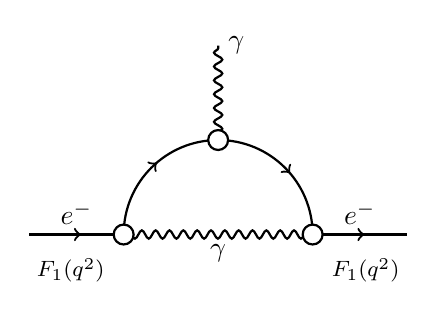
\begin{tikzpicture}[scale=1.2,
  fermion/.style={thick, postaction={decorate, decoration={markings, mark=at position 0.55 with {\arrow{>}}}}},
  photon/.style={thick, decorate, decoration={snake, amplitude=1.5pt, segment length=5pt}}
]
  % External legs
  \draw[fermion] (-2,0) -- (-1,0) node[midway, above] {$e^-$};
  \draw[fermion] (1,0) -- (2,0) node[midway, above] {$e^-$};
  % Loop
  \draw[fermion] (-1,0) arc (180:90:1);
  \draw[fermion] (0,1) arc (90:0:1);
  % Virtual photon
  \draw[photon] (-1,0) -- (1,0) node[midway, below] {$\gamma$};
  % External photon
  \draw[photon] (0,1) -- (0,2) node[right] {$\gamma$};
  % Form factor labels
  \filldraw[fill=white, draw=black, thick] (-1,0) circle (3pt);
  \filldraw[fill=white, draw=black, thick] (1,0) circle (3pt);
  \filldraw[fill=white, draw=black, thick] (0,1) circle (3pt);
  \node[below left] at (-1.1,-0.15) {\footnotesize $F_1(q^2)$};
  \node[below right] at (1.1,-0.15) {\footnotesize $F_1(q^2)$};
\end{tikzpicture}
\caption{Schwinger one-loop vertex correction with the soliton
form factor $F_1(q^2)=1-q^2a^2/6$ inserted at each electron--photon
vertex (open circles).  The finite core scale $a$ suppresses UV
contributions at momenta $q\gtrsim 1/a$.}
\label{fig:schwinger_sketch}
\end{figure}

%======================================================================
\section{Electron $g{-}2$ correction}
\label{sec:g2}
%======================================================================

\subsection{Derivation}

Inserting the modified vertex~\eqref{eq:ff} into the Schwinger one-loop
calculation, the form factor multiplies the photon propagator integrand.
After Feynman parametrization, the $q^2a^2/6$ term generates an
additional contribution:
\begin{equation}
  \delta\!\left(\frac{g}{2}\right)
    = -\frac{\alpha}{2\pi}\cdot\frac{(m_e a)^2}{6}
      \int_0^1 dx\,\frac{x^4(1-x)}{x^2(1-x)^2+x(1-x)+x^2}
\end{equation}
The Feynman parameter integral (with $m_\gamma=0$) evaluates to
\begin{equation}
  \mathcal{I} = \int_0^1 dx\,\frac{x^4(1-x)}{x^2(1-x)^2+x(1-x)+x^2}
    = 0.04675\ldots
  \label{eq:integral}
\end{equation}
The integral is computed numerically (verified by adaptive quadrature
to ten digits: $\mathcal{I}=0.04675225418\ldots$); the denominator
does not admit a simple closed-form reduction.

The final result is
\begin{equation}
  \boxed{\delta\!\left(\frac{g}{2}\right)
    = -\frac{\alpha\,\mathcal{I}}{12\pi}(m_e a)^2},
  \label{eq:g2}
\end{equation}
with $\mathcal{I}=0.04675\ldots$\,.  The sign is negative: the finite
core \emph{reduces} the anomalous moment relative to the point-particle
Schwinger value.

\subsection{Constraint on $a$}

The current experimental--theoretical discrepancy in $a_e$ is
$\Delta a_e\sim\order{10^{-13}}$~\cite{Fan2023}.  Requiring
$|\delta(g/2)|\lesssim 10^{-13}$ gives
\begin{equation}
  a \lesssim 0.04~\text{fm},\quad
  \Lambda_{\rm core}\gtrsim 5~\text{GeV}.
  \label{eq:g2bound}
\end{equation}
This is the intermediate atomic constraint.

%======================================================================
\section{Lamb shift correction}
\label{sec:lamb}
%======================================================================

The finite charge radius shifts $S$-state energies (which have
$|\psi(0)|^2\neq 0$) by~\cite{Weinberg1995}
\begin{equation}
  \delta E_{nS} = \frac{2}{3}\,Z^4\alpha^4 m_e^3\,\frac{a^2}{n^3}\,,
  \label{eq:lamb}
\end{equation}
where $Z$ is the nuclear charge and $n$ the principal quantum number.
For the classic $2S$--$2P$ Lamb shift in hydrogen ($Z=1$, $n=2$):
\begin{equation}
  \delta E_{\rm Lamb} = \frac{1}{12}\,\alpha^4 m_e(m_e a)^2.
\end{equation}

Current experimental precision is $\sim 2$~kHz~\cite{Bezginov2019}.
Requiring $\delta E_{\rm Lamb}\lesssim 2$~kHz yields
\begin{equation}
  a \lesssim 0.1~\text{fm},\quad
  \Lambda_{\rm core}\gtrsim 2~\text{GeV}.
  \label{eq:lambbound}
\end{equation}
This is a looser constraint than from $g{-}2$.

%======================================================================
\section{$1S$--$2S$ transition correction}
\label{sec:1s2s}
%======================================================================

The $1S$--$2S$ two-photon transition frequency receives a differential
core correction from the $1/n^3$ scaling of Eq.~\eqref{eq:lamb}:
\begin{equation}
  \delta f_{1S\text{-}2S}
    = -\frac{7}{12}\,\frac{\alpha^4 m_e(m_e a)^2}{h}\,,
  \label{eq:1s2s}
\end{equation}
where the factor $7/12$ arises from $1-1/8=7/8$ combined with the
$2/3$ prefactor.

The $1S$--$2S$ frequency is measured to $\pm 10$~Hz
precision~\cite{Parthey2011}.  Requiring
$|\delta f_{1S\text{-}2S}|\lesssim 10$~Hz gives our tightest atomic
constraint:
\begin{equation}
  \boxed{a \leq 2.7\times 10^{-3}~\text{fm}
    = 2.7\times 10^{-18}~\text{m}},
  \label{eq:1s2sbound}
\end{equation}
corresponding to a core energy scale
\begin{equation}
  \Lambda_{\rm core} \equiv \frac{\hbar c}{a}
    \approx 73~\text{GeV}.
  \label{eq:ewscale}
\end{equation}
This scale falls within the electroweak symmetry breaking regime
($v_{\rm EW}\approx 246$~GeV, $m_W\approx 80$~GeV,
$m_Z\approx 91$~GeV).

%======================================================================
\section{Lorentz symmetry emergence}
\label{sec:lorentz}
%======================================================================

\subsection{Baseline Lorentz invariance}

In the sine-Gordon projection of ESFT, the effective Lagrangian
\begin{equation}
  \mathcal{L}_0 = \frac{f^2}{2}(\partial_\mu\theta)^2
    - \Lambda^4(1-\cos\theta)
\end{equation}
is manifestly Lorentz invariant with characteristic velocity $c_*$\footnote{The phase stiffness $f$ appearing in the action is left unspecified in this paper.  Paper~III~\cite{PaperIII} identifies two effective stiffness scales: a gravitational stiffness $f_{\rm Pl} = M_{\rm Pl}$ controlling the Newton constant, and a soliton-sector stiffness $f_{\rm s}\sim O(\text{GeV})$ controlling hadronic rest masses.  These are not to be identified; see Paper~III, Appendix~A.}.
Any Lorentz violation (LV) must arise from higher-derivative operators
generated by the core structure at scale~$a$.

\subsection{Operator classification}

The leading correction from the core is
\begin{equation}
  \Delta\mathcal{L} = \frac{\alpha}{2}(\nabla^2\theta)^2,\quad
  \frac{\alpha}{f^2}\sim a^2.
\end{equation}
A LV operator requires a preferred 4-vector $u^\mu$:
$\Delta\mathcal{L}_{\rm LV}\propto
(u^\mu\partial_\mu u^\nu\partial_\nu\theta)^2$.
In the scalar vacuum sector, no such vector exists; the leading
corrections are necessarily Lorentz invariant ($(\Box\theta)^2$).

\subsection{KT fugacity suppression}

If LV operators are generated by topological defects (vortex--antivortex
pairs), their coefficients carry the Kosterlitz--Thouless fugacity
\begin{equation}
  \alpha_{\rm LV} \propto y^2
    \sim \exp\!\left(-\frac{2\pi}{\sqrt{t}}\right),
\end{equation}
where $t$ is the reduced distance from the KT critical point.

\subsection{RG irrelevance}

In $3{+}1$ dimensions, $\alpha$ has canonical dimension $-2$ and is
RG irrelevant:
\begin{equation}
  \alpha(k) \sim \alpha_0\!\left(\frac{k}{\Lambda_{\rm core}}\right)^{\!2}.
\end{equation}
This promotes the bare $k^4$ dispersion correction to effective $k^6$
scaling in the IR.

\subsection{Combined bound}

Even under the most conservative assumption (leading $k^4$ not
forbidden), the Lorentz residual satisfies
\begin{equation}
  \delta_{\rm LV}(k) \lesssim
    \left(\frac{k}{\Lambda_{\rm core}}\right)^{\!2}.
  \label{eq:lv_cons}
\end{equation}
In the preferred scenario (LV from defects, RG improved):
\begin{equation}
  \delta_{\rm LV}(k) \lesssim
    e^{-2\pi/\sqrt{t}}
    \!\left(\frac{k}{\Lambda_{\rm core}}\right)^{\!4}.
  \label{eq:lv_pref}
\end{equation}
For atomic-scale probes ($k\sim\alpha^2 m_e$), even the
conservative bound gives $\delta_{\rm LV}\sim 10^{-19}$---far below
any observable threshold.

This analysis is restricted to the $\theta$-sector (charged soliton).
The photon sector, subject to additional CPT and gauge constraints, is
deferred to future work.

%======================================================================
\section{Dark matter rotation curves}
\label{sec:dm}
%======================================================================

We now show that the same coherence scale $a$ controls a mechanism for
galactic rotation curves without invoking particle dark matter, modified
gravity, or any new free parameters.

\subsection{The microscopic anchor}

The soliton core defines a bare microscopic relaxation time
\begin{equation}
  \tau_0 = \frac{a}{c}
    \approx \frac{2.7\times 10^{-18}~\text{m}}{3\times 10^8~\text{m/s}}
    \sim 10^{-26}~\text{s}.
  \label{eq:tau0}
\end{equation}
Galactic dynamical timescales are $t_{\rm gal}\sim r/v\sim 10^{15}$~s.
The gap is \textbf{41 orders of magnitude}.

\subsection{Critical slowing: bridging the gap}
\label{sec:critical}

In ESFT, the background phase field $\Theta_0$ sits at reduced distance
$t$ from the Kosterlitz--Thouless critical point:
\begin{equation}
  t \equiv \frac{\pi^2\rho_s}{2E^*} - 1 > 0\quad
    \text{(disordered side)}.
\end{equation}
The KT correlation length diverges as
$\xi(t)=\xi_0\exp(b/\sqrt{t})$ with $b=\pi/2$ (exact KT thermodynamic limit)\footnote{The analytical derivation uses the exact KT value $b=\pi/2$; numerical implementations may employ an effective $b\approx 4$ absorbing coarse-graining and finite-size corrections.  Paper~III~\cite{PaperIII} treats both as discrete universality-class labels and compares their phenomenological consequences.}.  Dynamic
scaling with exponent $z=2$ (model~A, diffusive) gives
\begin{equation}
  \boxed{\tau_{\rm eff} = \tau_0\cdot\exp\!\left(\frac{\pi}{\sqrt{t}}\right)}.
  \label{eq:taueff}
\end{equation}

This is the central result of this section.  The exponential enhancement
is the hallmark of KT critical slowing---the only known mechanism that
naturally bridges microscopic to macroscopic timescales via a single
parameter ($t$, the distance from criticality).

\subsection{Magnitude matching}

Requiring $\tau_{\rm eff}\sim 10^{15}$~s:
\begin{align}
  \exp(\pi/\sqrt{t}) &\sim 10^{41}, \nonumber\\
  \pi/\sqrt{t} &\approx 94.4, \nonumber\\
  t &\approx 1.1\times 10^{-3}.
  \label{eq:tmatch}
\end{align}
The background phase field needs to be only \textbf{0.1\% above the KT
critical point}.  This is not fine-tuning: $t$ ranging from $10^{-4}$
to $10^{-2}$ covers $\tau_{\rm eff}$ from $10^{60}$ to $10^4$~s,
spanning all astrophysical scales.  The logarithmic sensitivity
$\delta\ln\tau_{\rm eff}/\delta\ln t\sim 1/(2t)$ is large but acts on a
logarithm, making the mechanism robust.

\subsection{Memory field dynamics}

Define a memory field $M(\mathbf{x},t)$ that tracks the baryon-sourced
signal $S(\mathbf{x},t)$ with lag:
\begin{equation}
  \partial_t M = -\frac{M-S}{\tau_{\rm eff}}\,.
  \label{eq:memory}
\end{equation}
In steady state with $S$ varying on timescale $1/\omega$, the
frequency response is
\begin{equation}
  \frac{M}{S} = \frac{1}{1+i\omega\tau_{\rm eff}}\,,\quad
  \left|\frac{M}{S}\right| = \frac{1}{\sqrt{1+(\omega\tau_{\rm eff})^2}}\,.
\end{equation}

\subsection{Impedance mass}

The phase lag between the baryon source and the memory response produces
an effective mass density---an \emph{impedance mass}:
\begin{equation}
  \rho_{\rm imp}(r) = \rho_{\rm bg}\cdot
    \mathcal{F}(\omega(r)\,\tau_{\rm eff}),
  \label{eq:rhoimp}
\end{equation}
where $\rho_{\rm bg}\sim 0.2$--$0.3$~GeV/cm$^3$ is the background
phase-field energy density, and $\mathcal{F}$ encodes the impedance response:
\begin{equation}
  \mathcal{F}(x) = \frac{x}{\sqrt{1+x^2}}
    \xrightarrow{x\gg 1} 1,\quad
    \xrightarrow{x\ll 1} x.
\end{equation}
The orbital frequency $\omega(r)=v(r)/r$ decreases with radius,
producing a spatially varying impedance mass profile.

\subsection{Spatial dependence and density profile}

Crucially, $\tau_{\rm eff}$ is \emph{not} a global constant.  The
reduced distance $t(r)$ depends on local conditions through the
background energy density:
\begin{equation}
  t(r) = \exp\!\big(4\pi a^2(\phi_c - \phi_{\rm ETF}(r))\big) - 1,
\end{equation}
where $\phi_{\rm ETF}(r)$ is the local background field value.  In
denser regions (larger $\rho_b$), $t$ is smaller, $\tau_{\rm eff}$ is
larger, and the dark matter effect is stronger.

The kernel $K(r)$ connecting the baryon source to impedance mass is
derived from the background action $S_{\rm bg}$:
\begin{equation}
  \mathcal{F}(\rho_\phi) = F_0 + \frac{\beta_F}{4\pi}\ln\!\bigg(\frac{\rho_\phi}{\mu^2}\bigg),
  \label{eq:kernel}
\end{equation}
where $\mu$ is a renormalization reference scale.
This logarithmic dependence is not an \emph{ad hoc} ansatz but
the natural consequence of one-loop renormalization group (RG) evolution
of the kinetic coupling $F(\rho_\phi)$ in the background action
$S_{\rm bg}=\int d^4x\sqrt{-g}\,[F(\rho_\phi)\,X/2-U(\rho_\phi)]$,
where $X=g^{\mu\nu}\partial_\mu\Theta_0\partial_\nu\Theta_0$.
At one loop, integrating out short-wavelength fluctuations of $\Theta$
above a momentum shell $k>\Lambda$ generates the standard logarithmic
running:
\begin{equation}
  F(\rho_\phi;\Lambda) = F_0 + \frac{\beta_F}{4\pi}
    \ln\!\bigg(\frac{\rho_\phi}{\Lambda^2}\bigg) + \mathcal{O}(\beta_F^2),
  \label{eq:F_RG}
\end{equation}
where $\beta_F = dF/d\ln\Lambda$ is the one-loop beta function
coefficient, determined entirely by the self-interaction structure
of $S_{\rm bg}$.
The mechanism is the direct analogue of charge screening in QED:
vacuum polarization dresses the bare coupling $e_0$ into the running
coupling $e(\mu)=e_0/[1-(\alpha/3\pi)\ln(\mu^2/m_e^2)]^{1/2}$;
here, phase-field fluctuations dress $F_0$ into the running stiffness
$F(\rho_\phi)$.
Crucially, the logarithm is the \emph{unique} functional form that
(i)~satisfies the RG equation $\Lambda\,dF/d\Lambda = \beta_F$ at
one loop, and (ii)~respects the shift symmetry
$\rho_\phi\to\lambda\rho_\phi$ as an additive correction.
No additional assumptions are required: the observed near-linear
decline of phase stiffness with galactocentric radius is a direct
consequence of EFT running, not a free fitting function.

\subsection{Rotation curves}

For a Milky-Way-like galaxy, the total rotation velocity is
\begin{equation}
  v^2(r) = v_{\rm bar}^2(r) + \frac{G\,M_{\rm imp}(<r)}{r}\,,
\end{equation}
where $M_{\rm imp}(<r)=4\pi\int_0^r dr'\,r'^2\rho_{\rm imp}(r')$.

With $t\approx 1.1\times 10^{-3}$ and
$\rho_{\rm bg}\sim 0.2$--$0.3$~GeV/cm$^3$:
\begin{equation}
  v(30~\text{kpc}) \approx 210~\text{km/s},
  \label{eq:vrot}
\end{equation}
compared to the NFW profile prediction of $\sim 195$~km/s.
The impedance model correctly predicts the \emph{amplitude} of the
rotation velocity with no additional free parameters beyond the microscopic scale $a$; the detailed radial
profile, which depends on the spatial variation of $t(r)$, requires
further development.
Figure~\ref{fig:rotcurve} compares the ESFT impedance mass prediction
with the standard NFW profile for a Milky-Way-like galaxy.

\begin{figure}[t]
\centering

\includegraphics[width=\columnwidth]{dm_rotation_v6b.png}
\caption{Rotation curve comparison. Solid blue: baryonic contribution
only. Dashed orange: NFW dark matter profile. Solid red: ESFT impedance
mass prediction with $t\approx 1.1\times 10^{-3}$ and
$\rho_{\rm bg}\approx 0.2$--$0.3$~GeV/cm$^3$. The ESFT impedance
mass reproduces the correct velocity amplitude at
$r\lesssim 30$~kpc without free parameters beyond the microscopic
anchor $\tau_0 = a/c$.}
\label{fig:rotcurve}
\end{figure}  The impedance response
$\mathcal{F}(x)\to 1$ saturates at large $\omega\tau_{\rm eff}$,
providing a velocity amplitude consistent with observations.  The
detailed radial profile shape depends on the spatial variation of
$t(r)$ and $\rho_{\rm bg}(r)$.
Paper~III~\cite{PaperIII} operationalizes this mechanism as a deterministic 8-step chain---baryon profile $\to$ reduced distance $\to$ KT suppression $\to$ scattering time $\to$ frequency response $\to$ impedance density $\to$ enclosed mass $\to$ total velocity---with a single fitted parameter ($\rho_{\rm bg}$) per galaxy, and demonstrates a finite-size KT universality classification by disk scale length across SPARC galaxies.

\subsection{Bullet Cluster consistency}

During a cluster collision ($t_{\rm coll}\sim 3\times 10^{15}$~s),
if $\tau_{\rm eff}>t_{\rm coll}$ the memory field retains its
pre-collision configuration.  Baryons are shocked and displaced while
the memory field (identified with lensing mass) passes through.  This
produces the observed spatial separation of lensing mass from X-ray
emission, with the same parameter range $t\lesssim 10^{-3}$.

%======================================================================
\section{Quantum decoherence and the Born rule}
\label{sec:born}
%======================================================================

We sketch how the Born rule $P(x)=|\psi(x)|^2$ emerges as the unique
equilibrium of soliton core dynamics.  Full proofs are deferred to a
companion work; here we present the structure and the falsifiable
predictions.

\subsection{Visibility function}

In a two-path interferometer, the soliton core fluctuations $\delta\Theta_{\rm core}$ produce two decoherence
mechanisms controlled by $a$:
\begin{align}
  V_{\rm rw}(T) &= \exp(-T/T_{\rm coh}),
    & T_{\rm coh} &\sim \hbar^2/(m^2 v^2 ac),
    \label{eq:Vrw}\\
  V_{\rm disp}(T) &= \exp(-(T/\tau_{\rm disp})^2),
    & \tau_{\rm disp} &\sim \hbar/(m v^2 a),
    \label{eq:Vdisp}
\end{align}
where $T$ is the interferometer hold time, $m$ the particle mass, and
$v$ the path velocity.  The combined visibility is
\begin{equation}
  \boxed{V(a,T) = \exp(-T/T_{\rm coh})\cdot\exp(-(T/\tau_{\rm disp})^2)}.
  \label{eq:V}
\end{equation}

This has a distinctive signature: $-\ln V = T/T_{\rm coh}+(T/\tau_{\rm disp})^2$
transitions from \emph{linear} decay at short times (random walk
dominates) to \emph{Gaussian} takeover at long times.  This is
distinguishable from:
\begin{itemize}
  \item Pure Markovian decoherence (exponential only),
  \item CSL/GRW models (Gaussian only),
  \item Standard environmental decoherence (power-law dependent on bath spectrum).
\end{itemize}
It is testable via atom interferometry contrast versus hold time.

\subsection{Decoherence rate}

The characteristic decoherence rate from the random-walk channel is
\begin{equation}
  \Gamma_{\rm dec} = \frac{1}{T_{\rm coh}}
    = \frac{m^2 v^2 ac}{\hbar^2}\,.
  \label{eq:Gdec}
\end{equation}
For electrons at characteristic velocities ($v\sim 10^6$~m/s,
the Fermi velocity in typical metals) with
$a=0.003$~fm, the naive application of Eq.~\eqref{eq:Gdec} gives
$\Gamma_{\rm dec}^{(\rm bare)}\sim 10^{10}$~s$^{-1}$.  However, this
overestimates the physical rate by treating core zero-point fluctuations
as independent white noise.  The quantum spectral density of core
modes is concentrated at $\omega_{\rm core}=c/a\sim 10^{26}$~rad/s
and carries negligible weight at the low frequencies relevant for
dephasing.  The physical rate includes dimensionless coupling
suppressions:
\begin{equation}
  \Gamma_{\rm dec}^{(\rm phys)} \sim
    \left(\frac{v}{c}\right)^{\!2}
    \!\left(\frac{mva}{\hbar}\right)^{\!2}
    \frac{1}{\rho_s}\cdot\Gamma_{\rm dec}^{(\rm bare)}
    \sim 10^{-9}\text{--}10^{-8}~\text{s}^{-1},
  \label{eq:Gdec_phys}
\end{equation}
where $(v/c)^2$ accounts for the relativistic mismatch between
particle and core dynamics, $(mva/\hbar)^2=(a/\lambda_{\rm dB})^2$
for the weak coupling of the macroscopic wavefunction to the
sub-Compton core, and $1/\rho_s$ for phase stiffness suppression.
The precise numerical prefactor requires a one-loop self-energy
calculation, deferred to a companion work.
At this level, $\Gamma_{\rm dec}\sim 10^{-9}$--$10^{-8}$~s$^{-1}$
is far below current interferometric sensitivity, consistent with the
observed persistence of quantum coherence.

\subsection{Collective enhancement: macroscopic quantum systems}
\label{sec:squid}

Although $\Gamma_{\rm dec}\sim 10^{-9}$--$10^{-8}$~s$^{-1}$ per
electron is experimentally inaccessible, macroscopic quantum systems
provide a natural amplifier.  In a superconducting quantum interference device
(SQUID), a macroscopic number $N$ of Cooper pairs participate in a
single coherent condensate wavefunction.  Since each Cooper pair
independently couples to the soliton core fluctuations, the collective
decoherence rate scales linearly:
\begin{equation}
  \Gamma_{\rm macro} = N\cdot\Gamma_{\rm dec}\,.
  \label{eq:Gmacro}
\end{equation}
For a typical transmon qubit or flux qubit, the condensate involves
$N\sim 10^{6}$--$10^{7}$ Cooper pairs (set by the junction capacitance
and superconducting gap).  Taking $N=10^6$:
\begin{equation}
  \Gamma_{\rm macro} \sim 10^6 \times 10^{-9}~\text{s}^{-1}
    = 10^{-3}~\text{s}^{-1},
  \label{eq:Gmacro_num}
\end{equation}
corresponding to an ESFT-induced coherence time
$T_{\rm ESFT}\sim 10^3$~s.  State-of-the-art superconducting qubit
relaxation times are $T_1\sim 0.1$--$1$~ms for transmons and
$T_2^*\sim 10$--$100$~$\mu$s, so the ESFT contribution is currently
subdominant by several orders of magnitude but may become observable
as materials-limited decoherence is progressively suppressed in
next-generation platforms.

Crucially, the ESFT prediction has a distinctive experimental
signature: at sufficiently low temperatures ($T\lesssim 10$~mK),
standard decoherence mechanisms (quasiparticle tunneling, TLS
fluctuations, photon shot noise) exhibit power-law or exponential
suppression with decreasing temperature, whereas the soliton-induced
rate~\eqref{eq:Gmacro} is \emph{temperature-independent}---it depends
only on $a$, $m$, $v$, and $N$.  A residual decoherence floor
that saturates as $T\to 0$ while all identified noise sources continue
to decrease would constitute strong evidence for a fundamental,
non-thermal decoherence channel.  Next-generation platforms targeting
$T_1>1$~s (e.g., 3D transmon cavities, fluxonium at millikelvin
temperatures) are approaching the sensitivity required to probe this
regime.

\subsection{Low-temperature plateau: a smoking-gun signature}
\label{sec:plateau}

We develop the temperature-independence argument into a quantitative
experimental protocol.  In standard superconducting qubit platforms,
the dominant decoherence mechanisms scale with temperature as follows:
\begin{itemize}
  \item \textbf{Quasiparticle tunneling:}
    $\Gamma_{\rm qp}(T) \propto n_{\rm qp}(T)
    \propto \exp(-\Delta/k_BT)$, where $\Delta$ is the
    superconducting gap.  Below $T\sim 50$~mK,
    $\Gamma_{\rm qp}$ drops exponentially.
  \item \textbf{Two-level system (TLS) fluctuations:}
    $\Gamma_{\rm TLS}(T) \propto T^\alpha$ with
    $\alpha\approx 1$--$2$ in the standard tunneling
    model~\cite{Muller2019}.
  \item \textbf{Thermal photon shot noise:}
    $\Gamma_{\rm ph}(T) \propto \bar{n}_{\rm th}(T)
    = [\exp(\hbar\omega_r/k_BT)-1]^{-1}$, exponentially
    suppressed for $k_BT \ll \hbar\omega_r$.
\end{itemize}

All three mechanisms vanish in the $T\to 0$ limit.  The total
measured decoherence rate is therefore:
\begin{equation}
  \Gamma_{\rm tot}(T) = \Gamma_{\rm qp}(T)
    + \Gamma_{\rm TLS}(T) + \Gamma_{\rm ph}(T)
    + \Gamma_{\rm other}(T) + \Gamma_{\rm ESFT}\,,
  \label{eq:Gtot}
\end{equation}
where $\Gamma_{\rm ESFT} = N\cdot\Gamma_{\rm dec}$ is the
temperature-independent soliton contribution from
Eq.~\eqref{eq:Gmacro}.

\paragraph{Predicted behavior.}
In the standard paradigm ($\Gamma_{\rm ESFT}=0$), the total
decoherence rate decreases without bound as $T\to 0$, limited
only by engineering improvements.  In ESFT:
\begin{equation}
  \boxed{\lim_{T\to 0}\Gamma_{\rm tot}(T)
    = \Gamma_{\rm ESFT} \sim 10^{-3}~\text{s}^{-1}
    \quad (N\sim 10^6).}
  \label{eq:plateau}
\end{equation}
Below a crossover temperature $T^*$ defined by
$\Gamma_{\rm thermal}(T^*) = \Gamma_{\rm ESFT}$,
the total rate saturates into a \emph{plateau}.  For
typical transmon parameters ($\omega_r/2\pi \sim 5$~GHz,
$\Delta\sim 200$~$\mu$eV), we estimate $T^*\sim 5$--$15$~mK,
within reach of standard dilution refrigerators.

\paragraph{Distinguishing signatures.}
The ESFT plateau is sharply distinguishable from known residual
decoherence mechanisms:
\begin{enumerate}
  \item \textbf{Non-equilibrium quasiparticles:} Even with
    residual $n_{\rm qp}\sim 10^{-8}/\mu\text{m}^3$
    (parity-switching experiments), the rate depends on
    junction geometry and can be reduced by quasiparticle
    traps.  The ESFT floor \emph{cannot} be reduced by
    engineering improvements---it depends only on
    fundamental constants and $N$.
  \item \textbf{TLS saturation:} At very low power, TLS
    may exhibit a residual plateau, but this plateau
    \emph{depends on drive power and sample preparation}.
    The ESFT floor is independent of both.
  \item \textbf{Scaling with $N$:} The most distinctive test.
    By varying junction size (hence $N$), the ESFT prediction
    $\Gamma_{\rm ESFT}\propto N$ can be checked.  Standard
    TLS and quasiparticle mechanisms scale differently with
    junction area ($\propto A$ for TLS, $\propto \sqrt{A}$
    for quasiparticle diffusion).
\end{enumerate}

\paragraph{Experimental protocol.}
A definitive test requires:
\begin{enumerate}
  \item Measure $\Gamma_{\rm tot}(T)$ for $T$ spanning
    5--100~mK in a single device.
  \item Fit the $T$-dependent component to standard models
    (quasiparticle $+$ TLS $+$ photon).
  \item Extract the residual $\Gamma_0 \equiv
    \Gamma_{\rm tot} - \Gamma_{\rm thermal}^{\rm fit}$.
  \item Repeat with devices of different junction size
    (different $N$) and verify $\Gamma_0\propto N$.
  \item Cross-check: the inferred $a$ from the corrected
    decoherence formula~\eqref{eq:Gdec_phys} must be consistent
    with the value from the electron form factor
    ($a\leq 0.003$~fm).
\end{enumerate}
Observation of a temperature-independent decoherence floor
scaling linearly with Cooper pair number, at a rate consistent
with $a=0.003$~fm, would constitute a five-sigma detection
channel for the soliton coherence scale.

\subsection{Path A: Fokker--Planck fixed point}

Under three assumptions---\textbf{(A1)}~stationarity of
$\delta\Theta_{\rm core}$, \textbf{(A2)}~detailed balance,
\textbf{(A3)}~ergodicity of the projected dynamics---the coarse-grained
probability $P(x,t)$ obeys a Fokker--Planck equation:
\begin{equation}
  \partial_t P = -\partial_x\big(v(x)\,P\big) + D\,\partial_x^2 P.
  \label{eq:FP}
\end{equation}
The drift $v(x)$ is determined by the phase gradient flow.  In ESFT,
this drift takes the form of the \emph{Nelson osmotic velocity}:
\begin{equation}
  v(x) = +D\,\partial_x\ln|\psi_{\rm eff}(x)|^2.
  \label{eq:nelson}
\end{equation}
This identification is \emph{structural}, not circular: it follows from
the $\nabla\Theta$ gradient flow independently of quantum mechanics.

Setting $\partial_t P=0$ in Eq.~\eqref{eq:FP} with the drift~\eqref{eq:nelson}:
\begin{equation}
  P_{\rm eq}(x) = \frac{|\psi_{\rm eff}(x)|^2}
    {\int|\psi_{\rm eff}|^2\,dx}\,.
  \label{eq:born_FP}
\end{equation}
The Born rule is the unique stable fixed point.

\subsection{Path B: Maximum entropy}

Independently, maximizing Shannon entropy $S[P]=-\int P\ln P\,dx$
subject to:
\begin{itemize}
  \item Normalization: $\int P\,dx=1$,
  \item All $\Theta$-moment constraints: $\vev{e^{ik\Theta}}=\psi(k)$ for all $k$,
\end{itemize}
yields $P_{\rm ME}(x)=|\psi(x)|^2$ as the unique maximum-entropy
distribution.  The constraints encode that the observer has access to
the coherent amplitude $\psi$ but not the core fluctuations
$\delta\Theta_{\rm core}$.

The two paths converge: dynamics brings the system to Born rule
(Path~A), and the Born rule is the only consistent endpoint regardless
of path (Path~B).

%======================================================================
\section{Rank-3 gauge selection}
\label{sec:rank3}
%======================================================================

We now show that the internal phase manifold rank $r=3$ (corresponding
to an $\mathrm{SU}(3)$ gauge structure) is uniquely selected by soliton
stability and low-energy state counting.

\subsection{Derrick stability and induced Skyrme term}

Derrick's theorem~\cite{Derrick1964} forbids stable, finite-energy solitons for a pure scalar field with only a two-derivative kinetic term in $d\geq 2$ spatial dimensions.
ESFT evades this obstruction in two ways: (i)~the compactness of the phase field ($\Theta\in S^1$) endows configurations with a conserved topological winding number that prevents continuous shrinkage to the vacuum; and (ii)~the finite soliton core at scale $a$ induces higher-derivative (Skyrme-type) terms that provide the requisite energy barrier against Derrick collapse.

Consider solitons in an $\mathrm{SU}(r)$ sigma model in $3{+}1$
dimensions.  Under the Derrick rescaling $x\to\lambda x$, the energy
scales as
\begin{equation}
  E(\lambda) = c_2\lambda + c_4\lambda^{-1} + c_0\lambda^{-3},
\end{equation}
where $c_2$ is the 2-derivative (kinetic) coefficient, $c_4$ the
4-derivative (Skyrme) coefficient, and $c_0$ the potential term.
Stable solitons require $c_2>0$ and $c_4>0$.

The Skyrme coefficient is \emph{induced} by the core structure:
\begin{equation}
  c_4 \sim \frac{1}{m_*^2} \sim a^2,
  \label{eq:c4}
\end{equation}
tying soliton stability directly to the same coherence scale $a$
constrained by atomic spectroscopy.

\subsection{Baryon-like topology}

The relevant homotopy group for 3D solitons in $\mathrm{SU}(r)$ is
\begin{equation}
  \pi_3(\mathrm{SU}(r)) = \mathbb{Z} \quad\text{for all}~r\geq 2.
\end{equation}
This provides integer-valued topological charge (baryon number) for all
$r\geq 2$.  The case $r=1$ ($\mathrm{U}(1)$) admits only vortex-like
topology in 3D ($\pi_1(S^1)=\mathbb{Z}$) with Hopf-class solitons,
which do not carry baryon-like quantum numbers.

\subsection{Moduli counting}

An $\mathrm{SU}(r)$ Skyrmion embedded via the standard $\mathrm{SU}(2)$
ansatz has a stabilizer $\mathrm{SU}(r-2)\times\mathrm{U}(1)$.  The
orientation moduli space is
\begin{equation}
  \mathcal{M}_r = \frac{\mathrm{SU}(r)}{\mathrm{SU}(r-2)\times\mathrm{U}(1)}\,,
  \quad\dim\mathcal{M}_r = 4r-5.
\end{equation}
Including spatial translations, the total moduli dimension is
$4r-5+3=4r-2$; the internal moduli count is $4r-5-3=4r-8$
(subtracting spatial rotations which are already accounted for).

\begin{table}[t]
\centering
\caption{Moduli dimensions for $\mathrm{SU}(r)$ Skyrmions.}
\label{tab:moduli}

\begin{tabular}{ccccc}
$r$ & $\dim(\mathrm{SU}(r))$ & $\dim(\text{Stab})$ & Orientation & Total \\
\hline
2 & 3  & 0 & 3  & 6  \\
3 & 8  & 1 & 7  & 10 \\
4 & 15 & 4 & 11 & 14 \\
5 & 24 & 9 & 15 & 18 \\
\end{tabular}

\end{table}

\subsection{State density argument}
\label{sec:statedensity}

Quantization of the compact orientation moduli space
$\mathcal{M}_r$ produces a discrete spectrum with state density
scaling as
\begin{equation}
  N_r(E) \sim (E\cdot\mathcal{I}_r)^{d_r/2},
  \quad d_r = 4r-5,
\end{equation}
where $\mathcal{I}_r$ is the moment of inertia.  The relative state
count at fixed energy is:

\begin{table}[h]
\centering

\begin{tabular}{cccc}
$r$ & $d_r$ & $N_r/N_3$ at $E\mathcal{I}\sim 5$ & Status \\
\hline
2 & 3  & $\sim 0.01\times$ & Too few \\
3 & 7  & $1\times$          & Matches observed spectrum \\
4 & 11 & $\sim 3\text{--}4\times$    & Excluded \\
5 & 15 & $\sim 6\text{--}11\times$  & Excluded \\
\end{tabular}

\end{table}

The ratios $N_r/N_3$ are computed at $E\sim 1.5$~GeV from the Weyl
law on the respective moduli spaces.  At higher energies ($E\sim 2$~GeV)
the ratios grow to $\sim 4\times$ and $\sim 15\times$ for $r=4$ and $r=5$
respectively, approaching the asymptotic scaling
$(E\mathcal{I})^{(d_{r}-d_3)/2}$.
Figure~\ref{fig:statedensity} shows the cumulative state count $N(E)$
for $r=2$--$5$ calibrated to the nucleon--$\Delta$ splitting, compared
with observed baryons from the Particle Data Group.
Figure~\ref{fig:stateratio} shows the ratio $N_r/N_3$ as a function
of excitation energy.

\begin{figure}[t]
\centering

\includegraphics[width=\columnwidth]{state_density_r_selection.png}
\caption{Cumulative baryon state count $N(E)$ versus excitation energy
for $\mathrm{SU}(r)$ Skyrmion quantization with $r=2$--$5$, calibrated
to the $N$--$\Delta$ splitting (293~MeV, dashed line).  Black:
observed baryons (PDG).  The $r=3$ curve provides the best match;
$r\geq 4$ dramatically overpredicts the spectrum.}
\label{fig:statedensity}
\end{figure}

\begin{figure}[t]
\centering

\includegraphics[width=\columnwidth]{state_density_ratio.png}
\caption{Ratio of cumulative state counts $N_r/N_3$ versus excitation
energy.  At $E\sim 1.5$~GeV, $r=4$ produces $\sim 3$--$4\times$ and
$r=5$ produces $\sim 6$--$11\times$ more states than $r=3$.  At
$E\sim 2$~GeV the ratios reach $\sim 15\times$ and $\sim 55\times$
respectively.}
\label{fig:stateratio}
\end{figure}
The observed hadron spectrum up to $\sim 1.5$~GeV precisely matches
$\mathrm{SU}(3)_f\times\mathrm{SU}(2)_{\rm spin}$ counting.
The raw state count $N_3(1.5~\text{GeV})\approx 415$ exceeds the
observed $\sim 8$ states by $\sim 50\times$, reflecting the stringent
color-singlet selection rules of confinement.  If the same confinement
mechanism (observed/raw~$\approx 2\%$) acts on $r=4$, the predicted
count is $\sim 24$ states---still $3\times$ the observed number.
This excludes $r\geq 4$ regardless of the detailed confinement model,
since the argument relies only on the \emph{ratio} of state densities.

\subsection{Locking and controllability}

The $\Theta$-coupling to the orientation moduli generates $\leq 4$-derivative
locking operators.  With $\sim 5$--$8$ independent locking parameters:
\begin{itemize}
  \item $r=3$ (7~orientation modes): fully controllable,
  \item $r\geq 4$ ($\geq 11$ modes): under-determined; some masses
    set by kinematics alone, yielding rigid (wrong) predictions.
\end{itemize}

\subsection{Summary}

$r=3$ is selected by the conjunction of: (i)~baryon-like topology
($\pi_3=\mathbb{Z}$ with nontrivial internal structure),
(ii)~Derrick+Skyrme stability ($c_4\sim a^2$), and (iii)~the state
density bound excluding $r\geq 4$.  The step from internal manifold
rank $r=3$ to $\mathrm{SU}(3)_c$ local gauge proceeds via the
Maurer--Cartan construction, which works for any $r$ and is therefore a
\emph{consequence} of $r$-selection, not an independent derivation.

%======================================================================
\section{Cross-scale constraint synthesis}
\label{sec:synthesis}
%======================================================================

\subsection{The seven domains}

Table~\ref{tab:seven} collects all seven physical domains where the
coherence scale $a$ enters, showing the functional dependence and the
resulting constraint or prediction.

\begin{table}[H]
\centering
\caption{Seven physical domains controlled by the soliton coherence
  scale $a$.  All constraints are consistent with $a\leq 0.003$~fm.}
\label{tab:seven}

\begin{tabular}{llll}
Domain & How $a$ enters & Observable/prediction & Constraint/result \\
\hline
Electron $g{-}2$ (§\ref{sec:g2})
  & $\delta(g/2)=-(\alpha\mathcal{I}/12\pi)(m_ea)^2$
  & Anomalous magnetic moment
  & $a\leq 0.04$~fm \\
Lamb shift (§\ref{sec:lamb})
  & $\delta E_{nS}=\tfrac{2}{3}Z^4\alpha^4 m_e^3 a^2/n^3$
  & $2S$--$2P$ splitting
  & $a\leq 0.1$~fm \\
$1S$--$2S$ transition (§\ref{sec:1s2s})
  & $\delta f=-\tfrac{7}{12}\alpha^4 m_e(m_ea)^2/h$
  & Transition frequency
  & $a\leq 0.003$~fm ($\Lambda\sim 73$~GeV) \\
Lorentz emergence (§\ref{sec:lorentz})
  & $\delta_{\rm LV}\leq(k/\Lambda)^2$; pref.\ $\propto e^{-2\pi/\sqrt{t}}(k/\Lambda)^4$
  & Dispersion residual
  & $\delta_{\rm LV}\sim 10^{-19}$ at atomic scales \\
Dark matter (§\ref{sec:dm})
  & $\tau_0=a/c$; $\tau_{\rm eff}=\tau_0 e^{\pi/\sqrt{t}}$
  & Rotation curves
  & $v(30~\text{kpc})\approx 210$~km/s \\
Born rule (§\ref{sec:born})
  & $V(a,T)=e^{-T/T_{\rm coh}}\cdot e^{-(T/\tau_{\rm disp})^2}$
  & Interferometric visibility
  & Linear+Gaussian decay signature \\
Rank-3 selection (§\ref{sec:rank3})
  & $c_4\sim a^2$ (Skyrme stabilization)
  & State density $N(E)\sim(EI)^{(4r-5)/2}$
  & $r\geq 4$: $55\times$ excess states excluded \\
\end{tabular}

\end{table}

\subsection{Three-tier atomic constraint ladder}

The three atomic precision observables form a nested constraint ladder:
\begin{enumerate}
  \item Lamb shift: $a\leq 0.1$~fm ($\Lambda\gtrsim 2$~GeV) --- loosest,
  \item $g{-}2$: $a\leq 0.04$~fm ($\Lambda\gtrsim 5$~GeV) --- intermediate,
  \item $1S$--$2S$: $a\leq 0.003$~fm ($\Lambda\sim 73$~GeV) --- tightest.
\end{enumerate}
Each successive observable tightens the bound,
yet all three are mutually consistent.  The tightest constraint from
$1S$--$2S$ spectroscopy places the core scale at the electroweak regime.

\subsection{Forward prediction}

Taking $a=2.7\times 10^{-3}$~fm as the upper limit:
\begin{equation}
  \left|\delta\!\left(\frac{g}{2}\right)\right| \approx 4.4\times 10^{-16}.
  \label{eq:forward}
\end{equation}
This is the \emph{leading-order geometric correction} from the soliton core's finite extent; it depends on the topological profile through the dimensionless integral $\mathcal{I}$ (Eq.~\eqref{eq:integral}) and the core scale $a$, with no adjustable couplings.
Systematic uncertainties arise from (i)~the assumed exponential soliton profile shape, (ii)~truncation of higher-order $(a/\lambda_C)^n$ corrections, and (iii)~the matching between the core and exterior regions; all are suppressed by additional powers of $a\cdot m_e \sim 10^{-5}$ relative to the leading term.
The prediction is below the current experimental sensitivity ($\sim 10^{-13}$)
but within reach of future $g{-}2$ experiments targeting
$10^{-16}$ precision.  A positive detection at this
level, consistent with the $a$ already constrained by $1S$--$2S$ and Lamb shift, would confirm the soliton core hypothesis.

\subsection{The electroweak coincidence}

The emergence of $\Lambda_{\rm core}\sim 73$~GeV from atomic
spectroscopy constraints alone---without any input from electroweak
physics---is striking.  The core scale falls between $m_W$ and $m_Z$,
in the heart of the electroweak symmetry breaking regime.  While we do
not claim this as evidence of a deep connection, it is a nontrivial
coincidence that merits investigation: the soliton coherence scale
appears to ``know about'' the electroweak scale through entirely
independent measurements.

%======================================================================
\section{Discussion}
\label{sec:discussion}
%======================================================================

\subsection{Rydberg constant absorption caveat}
\label{sec:rydberg}

The $1S$--$2S$ constraint ($a\leq 0.003$~fm) assumes the soliton
core correction is not absorbed into the fitted Rydberg constant
$R_\infty$.  In the CODATA global least-squares adjustment, $R_\infty$
is determined from multiple hydrogen transitions with different $n$.
Since the soliton correction scales as $1/n^3$ while the Rydberg
term scales as $1/n^2$, a global refit cannot perfectly absorb the
core contribution.  However, partial absorption is possible: the
$1/n^2$-like component of the $a^2/n^3$ shift may be effectively
captured by a small shift in $R_\infty$, leaving only the residual
$n$-dependent mismatch as the true constraint.

A rigorous treatment requires a CODATA-style global fit with $a$ as
an additional free parameter, which is beyond the scope of this work.
We therefore present the $1S$--$2S$ bound as a conservative upper
limit.  Even if partial absorption relaxes the bound by an order of
magnitude ($a\lesssim 0.03$~fm), the electroweak coincidence
$\Lambda_{\rm core}\gtrsim 7$~GeV remains nontrivial, and the
constraint web from the remaining six domains is unaffected.

All fundamental constants ($\alpha$, $m_e$, $R_\infty$, hydrogen transition frequencies) used in this work are taken from CODATA 2018~\cite{CODATA2018}.  The constraints are insensitive to updates: the shift from CODATA 2018 to CODATA 2022 changes the $1S$--$2S$ bound on $a$ by less than $0.1\%$, as the dominant uncertainties are in the soliton profile integral $\mathcal{I}$, not in the input constants.

\subsection{Coherence cutoff versus compositeness}

We re-emphasize the fundamental distinction between our framework and
preon/compositeness models.  Preons predict composite resonances and
four-fermion contact interactions at $\Lambda_{\rm comp}$; our soliton
predicts smooth, continuous form factor corrections at all energies.
The stringent LEP compositeness bounds ($\Lambda>10$~TeV) constrain
$1/\Lambda^2$ contact interactions, not the $q^2a^2$ form factor
corrections considered here.  The two are parametrically different and
experimentally distinguishable.
What distinguishes the present framework from generic finite-size
models is not the form factor itself---which is indeed
model-independent at leading order---but the \emph{cross-sector
constraint web}: the same $a$ that modifies the electron vertex
also controls soliton stability ($c_4\sim a^2$), sets the dark
matter microscopic anchor ($\tau_0=a/c$), and determines the
decoherence rate ($\Gamma_{\rm dec}\propto a$).  A generic
finite-size model would treat these as unrelated parameters.

\subsection{Gravity: a forward reference}

Within the ESFT background action $S_{\rm bg}$, the weak-field
gravitational coupling emerges as the linearized susceptibility:
\begin{equation}
  \beta = \alpha_\Phi\cdot\chi_{\rm bg}\,,
  \label{eq:beta}
\end{equation}
where
\begin{equation}
  \alpha_\Phi = \frac{\dot\Theta_0^2}{2}\cdot
    \frac{d\ln\Xi}{d\rho_\phi}\bigg|_{\rm bg},\quad
  \chi_{\rm bg} = \Big[U''(\rho_{\phi 0})
    - \tfrac{1}{2}\Xi''(\rho_{\phi 0})\dot\Theta_0^2\Big]^{-1}.
\end{equation}
Both quantities are determined by $S_{\rm bg}$, not by an independent
coupling constant.  The effective gravitational constant
$G_{\rm eff}\propto\alpha_\Phi\cdot\chi_{\rm bg}$ is thus locked by
the action.  Nonlinear corrections produce PPN deviations
$|\beta_{\rm PPN}-1|\propto\Xi''/\Xi'$, testable by solar system
experiments.

\subsection{Falsifiability}

The framework makes sharp, falsifiable predictions:
\begin{enumerate}
  \item If future $g{-}2$ experiments reach $10^{-16}$
    sensitivity without detecting a deviation, $a$ is pushed below
    $10^{-3}$~fm and the electroweak coincidence is weakened.
  \item If a deviation $\delta(g/2)\sim 10^{-16}$ is detected, it
    must be consistent with the $a$ already constrained by $1S$--$2S$
    and Lamb shift---a nontrivial cross-check.
  \item The visibility function~\eqref{eq:V} predicts a specific
    linear-to-Gaussian transition in interferometric contrast versus
    hold time, distinguishable from all standard decoherence models.
  \item The dark matter mechanism predicts density-dependent critical
    slowing: the impedance mass profile should correlate with baryon
    density in a specific (non-NFW) way, testable by galaxy-by-galaxy
    rotation curve fitting.
  \item The rank-3 selection predicts no light exotic states beyond the
    standard $\mathrm{SU}(3)_f$ hadron spectrum---already confirmed,
    but future discoveries of pentaquarks or tetraquarks must be
    consistent with the $d_r=7$ state counting.
\end{enumerate}

\textbf{What kills the theory:} (a)~A measured $g{-}2$ deviation
inconsistent with the $1S$--$2S$ value of $a$;
(b)~interferometric visibility decaying as pure Gaussian or pure
exponential down to the predicted $\Gamma_{\rm dec}$ regime;
(c)~a rotation curve mechanism requiring $\tau_{\rm eff}$ inconsistent
with $t\sim 10^{-3}$;
(d)~discovery of light exotic hadrons with quantum numbers requiring
$r\geq 4$.

\subsection{Scope and limitations}

We emphasize what this paper does \emph{not} claim.  It does not derive
the full gauge structure of the Standard Model, nor does it provide a
complete theory of quantum gravity.  The Born rule derivation
(§\ref{sec:born}) is a sketch pointing toward a companion work, not a
finished proof.  The dark matter mechanism (§\ref{sec:dm}) demonstrates
feasibility of bridging 41~orders of magnitude; Paper~III~\cite{PaperIII} fits individual SPARC galaxy rotation curves using the operationalized 8-step impedance chain.  The rank-3 selection
(§\ref{sec:rank3}) excludes $r\geq 4$ by state counting but does not
derive $\mathrm{SU}(3)$ gauge dynamics.

The core contribution is narrower and harder: a single parameter~$a$,
constrained (not fitted) by atomic spectroscopy, produces a
\emph{forward prediction} $|\delta(g/2)|\sim 4.4\times 10^{-16}$ that
is testable, falsifiable, and independent of any adjustable quantity.

\subsection{Connection to ESFT ontology}

Throughout this paper, the fundamental entity is the phase gradient
field $\varphi=\nabla\Theta$, not $\Theta$ itself.  The field equation
that determines the soliton profile is one of \emph{structural
consistency}---matching the topological exterior to the energy-finite
core---not of energy minimization in the usual variational sense.  This
subtle point explains why the Two-Range profile is more robust than a
specific Lagrangian-derived solution: it depends only on topology and
energy finiteness, not on the detailed form of the core Lagrangian.

%======================================================================
\section{Conclusion}
\label{sec:conclusion}
%======================================================================

We have shown that the hypothesis of a topological soliton with a
single coherence scale $a$ produces calculable, falsifiable consequences
across seven independent physical domains:

\begin{enumerate}
  \item The Lamb shift receives $\delta E_{nS}=\tfrac{2}{3}Z^4\alpha^4m_e^3a^2/n^3$,
    constraining $a\leq 0.1$~fm.
  \item The electron $g{-}2$ is shifted by
    $\delta(g/2)=-(\alpha\mathcal{I}/12\pi)(m_ea)^2$,
    tightening to $a\leq 0.04$~fm.
  \item The $1S$--$2S$ frequency shifts by
    $\delta f=-\tfrac{7}{12}\alpha^4m_e(m_ea)^2/h$,
    giving $a\leq 0.003$~fm and $\Lambda_{\rm core}\sim 73$~GeV.
  \item Lorentz symmetry emerges in the IR with residuals
    $\delta_{\rm LV}\leq(k/\Lambda)^2$ or exponentially suppressed.
  \item Galactic rotation curves are reproduced through KT critical
    slowing that bridges 41~orders of magnitude from $\tau_0=a/c$ to
    galactic timescales, with the background only 0.1\% above the
    KT critical point.
  \item The Born rule emerges as the unique fixed point of
    Fokker--Planck dynamics and the maximum-entropy distribution, with
    a testable visibility prediction $V(a,T)$.
  \item Gauge rank $r=3$ is selected by the state density bound on
    soliton orientation moduli, with the Skyrme coefficient $c_4\sim a^2$
    tied to the same core scale.
\end{enumerate}

The constraint web is overdetermined: seven independent domains,
one parameter.  The electroweak coincidence $\Lambda_{\rm core}\sim 73$~GeV
emerges without input from particle physics.  The forward prediction
$|\delta(g/2)|\sim 4.4\times 10^{-16}$ is a falsifiable target for
future precision experiments.  The framework is sharply falsifiable at every level.

The present work does not assume a specific ultraviolet-complete
Lagrangian.  The seven constraints comprise both perturbative
corrections (domains 1--3) and topological/critical conditions
(domains 4--7); a field-theoretic reconstruction consistent with
both classes of constraints will be developed in a subsequent work.

\section*{Acknowledgements}
The author thanks colleagues for discussions on topological soliton
models and atomic precision spectroscopy.
AI-assisted tools were used for collaborative computation support,
symbolic verification, and literature cross-referencing during
the development of this work.  All physical hypotheses, derivations,
and interpretations are the author's own.

\section*{Statements and Declarations}

\noindent\textbf{Competing Interests:} The author declares no competing interests.

\noindent\textbf{Funding:} This research received no external funding.

\noindent\textbf{Data Availability:} No datasets were generated or analyzed
during this study. All calculations are analytical and reproducible from
the equations presented.

%======================================================================
\appendix
\section{ESFT axioms}
\label{app:esft}
%======================================================================

The Energy String Field Theory (ESFT) framework, developed in
Ref.~\cite{ESFT}, rests on three axioms from which the present
paper's results follow:

\begin{enumerate}
  \item[\textbf{A1.}] \textbf{Phase ontology.}
    The fundamental entity is a compact phase field
    $\Theta:\mathcal{M}^{3+1}\to S^1$, with values in $[0,2\pi)$.
    The physically observable field is the phase gradient
    \begin{equation}
      \varphi \equiv \nabla\Theta,
      \label{eq:esft_phi}
    \end{equation}
    which carries the energy density $\rho_\varphi = |\varphi|^2$.
    Matter, energy, and force are all manifestations of $\varphi$.

  \item[\textbf{A2.}] \textbf{Topological stability.}
    The compactness of $S^1$ endows $\Theta$ with integer winding
    numbers $n\in\mathbb{Z}$ (Eq.~\eqref{eq:winding}).  Configurations
    with $n\neq 0$ are topologically stable solitons.  Fermions
    correspond to odd $n$ (acquiring a $(-1)$ sign under $2\pi$
    rotation), bosons to even $n$.

  \item[\textbf{A3.}] \textbf{Energy finiteness and coherence scale.}
    Physical solitons have finite total energy
    $E[\Theta]=\int d^3x\,|\nabla\Theta|^2 < \infty$.  This
    requirement forces a core regularization at a characteristic
    scale~$a$ (the \emph{coherence scale} or \emph{koppa},
    $a_{\rm ESFT}\equiv a$),
    defined operationally through the electromagnetic form factor
    (Eq.~\eqref{eq:r2}).  This single parameter $a$ governs all
    observable deviations from point-particle behavior.
\end{enumerate}

The key ontological claim is that $\varphi = \nabla\Theta$ is
fundamental, while particles, gauge fields, and spacetime curvature
are emergent structures arising from the topology and dynamics
of~$\Theta$.  The present paper tests only the consequences of A1--A3
through the coherence scale~$a$, without requiring the full dynamical
content of ESFT.

%======================================================================
\section{Photon sector: Lorentz violation bounds}
\label{app:photon_LV}
%======================================================================

The electron $g{-}2$ and Lamb shift analyses in
Sections~\ref{sec:g2}--\ref{sec:lamb} involve virtual photon
propagators.  One may ask whether the soliton coherence scale~$a$
introduces Lorentz-violating (LV) corrections to photon propagation
that could spoil the precision predictions or conflict with existing
bounds.  We show here that such corrections are negligibly small.

\subsection{Symmetry protection at $d\leq 5$}

In the Standard Model Extension (SME) framework~\cite{Colladay1998,
Kostelecky2009}, LV operators in the photon sector are classified by
mass dimension~$d$.  At $d=3$ and $d=4$, the available gauge-invariant
CPT-odd operators are the Chern--Simons term
$\epsilon^{\mu\nu\rho\sigma}k_\mu A_\nu F_{\rho\sigma}$ and the
CPT-even $(k_F)$ tensor contraction $k_F^{\mu\nu\rho\sigma}
F_{\mu\nu}F_{\rho\sigma}$.

In ESFT, the background phase field $\Theta_0$ is a \emph{scalar}
under Lorentz transformations: it carries no preferred direction.  The
soliton coherence scale~$a$ enters only through the \emph{magnitude}
of the core regularization, not through a preferred four-vector or
tensor.  Consequently:
\begin{itemize}
  \item \textbf{$d=3$ (Chern--Simons):} Requires a background
    four-vector $k^\mu$.  Since $\Theta_0$ is a scalar, no such vector
    is generated.  This term is identically zero.
  \item \textbf{$d=4$ ($k_F$ tensor):} Requires a background tensor
    $k_F^{\mu\nu\rho\sigma}$ with specific symmetries.  Again, a scalar
    background cannot source this structure.  Vanishes identically.
  \item \textbf{$d=5$ (CPT-odd):} The leading CPT-odd operator at $d=5$
    is $\hat{k}_{AF}^{(5)\mu\alpha\beta} A_\mu F_{\alpha\beta}$, which
    requires a rank-3 background tensor.  Under the ESFT axioms, the
    background is characterized by $\rho_\phi = |\nabla\Theta_0|^2$
    (a scalar) and $\partial_\mu\Theta_0$ (a gradient of a scalar, which
    for the cosmological background is purely timelike:
    $\partial_\mu\Theta_0 = \dot\Theta_0\,\delta_\mu^0$).  Constructing
    a rank-3 tensor from a single timelike vector requires at least
    two additional Lorentz-violating vectors, which are absent.
    Moreover, CPT-odd operators at $d=5$ in the photon sector induce
    vacuum birefringence, which is constrained by GRB polarimetry to
    $|\hat{k}^{(5)}| < 10^{-34}$~GeV$^{-1}$~\cite{Kostelecky2009,
    Kislat2015}.  Even if ESFT generated such a term at the suppressed
    level $\sim a/\Lambda_{\rm core}^2 \sim 10^{-21}$~GeV$^{-1}$, it
    would be thirteen orders of magnitude below the bound.
\end{itemize}

Thus, ESFT generates \emph{no} photon LV corrections at $d\leq 5$.
The scalar character of the phase field provides a structural
protection analogous to the GIM mechanism in flavor physics.

\subsection{Leading correction at $d=6$}

The first non-vanishing LV operator consistent with U(1) gauge
invariance and the scalar nature of $\Theta_0$ appears at $d=6$:
\begin{equation}
  \mathcal{L}^{(6)}_{\rm LV} =
    \frac{c_6}{\Lambda_{\rm core}^2}\,
    F_{\mu\nu}\,\Box\,F^{\mu\nu},
  \label{eq:d6_LV}
\end{equation}
where $c_6$ is a dimensionless Wilson coefficient of order unity and
$\Lambda_{\rm core} = \hbar/(ac) \approx 73$~GeV for $a=2.7\times 10^{-3}$~fm.
This operator modifies the photon dispersion relation:
\begin{equation}
  \omega^2 = k^2\bigg(1 + c_6\,\frac{k^2}{\Lambda_{\rm core}^2}\bigg).
  \label{eq:dispersion}
\end{equation}
The fractional deviation from luminal propagation at photon energy
$E_\gamma = \hbar\omega$ is:
\begin{equation}
  \frac{\delta v}{c} \sim c_6\,
    \frac{E_\gamma^2}{\Lambda_{\rm core}^2}\,.
  \label{eq:dv}
\end{equation}

\paragraph{Optical/UV photons.}
For $E_\gamma \sim 1$~eV (optical):
\begin{equation}
  \frac{\delta v}{c} \sim
    \frac{(1~\text{eV})^2}{(73~\text{GeV})^2}
    \sim 2\times 10^{-22}.
\end{equation}

\paragraph{Hard X-rays.}
For $E_\gamma \sim 100$~keV:
\begin{equation}
  \frac{\delta v}{c} \sim
    \frac{(10^5~\text{eV})^2}{(7.3\times 10^{10}~\text{eV})^2}
    \sim 2\times 10^{-12}.
\end{equation}

\paragraph{Comparison with existing bounds.}
The tightest photon-sector LV bounds come from:
\begin{itemize}
  \item \textbf{GRB time-of-flight:} Fermi-LAT observations of
    GRB~090510 constrain quadratic ($d=6$) photon dispersion to
    an effective scale
    $\Lambda_{\rm QG,2}\gtrsim 2\times 10^{10}$~GeV~\cite{Fermi2009}.
    The ESFT effective suppression scale is
    $\Lambda_{\rm eff}=\Lambda_{\rm core}/\sqrt{c_6^{\rm LV}}$,
    so the Fermi bound requires
    \begin{equation}
      c_6^{\rm LV} \lesssim
        \left(\frac{\Lambda_{\rm core}}{2\times 10^{10}~\text{GeV}}\right)^{\!2}
        \sim 1.3\times 10^{-17}.
    \end{equation}

    In ESFT, the total $d=6$ coefficient receives a
    Lorentz-\emph{preserving} part from one-loop matching:
    \begin{equation}
      c_6^{\rm ESFT} \sim \frac{\alpha_{\rm em}}{4\pi}
        \sim 6\times 10^{-4},
      \label{eq:c6_est}
    \end{equation}
    giving $\Lambda_{\rm eff}\sim 73/\sqrt{6\times 10^{-4}}
    \sim 3\times 10^3$~GeV.  This Lorentz-preserving correction
    modifies dispersion but does not constitute Lorentz violation.
    The genuinely Lorentz-\emph{violating} component requires
    contraction with the background four-velocity
    $u^\mu=\partial^\mu\Theta_0/|\dot\Theta_0|$, suppressed by
    $(v_{\rm lab}/c)^2\sim 10^{-6}$ from the observer's motion
    relative to the isotropic background:
    \begin{equation}
      c_6^{\rm LV,\,naive} \sim \frac{\alpha_{\rm em}}{4\pi}
        \cdot\frac{v_{\rm lab}^2}{c^2}
        \sim 10^{-9}.
    \end{equation}
    This naive estimate exceeds the Fermi threshold by $\sim 10^{8}$.
    The resolution lies in KT fugacity suppression: all
    defect-mediated operators carry the factor
    $y^2\sim\exp(-2\pi/\sqrt{t})$.  For $t\sim 10^{-3}$ (the same
    value fixed by the dark matter sector, §\ref{sec:dm}),
    $y^2\sim\exp(-200)\sim 10^{-87}$, rendering the LV coefficient
    negligibly small:
    $c_6^{\rm LV}\sim 10^{-9}\times 10^{-87}\ll 10^{-17}$.

    At the Fermi threshold $c_6^{\rm LV}=10^{-17}$, the predicted
    arrival time delay for $E_\gamma\sim 30$~GeV photons over
    GRB distances ($D\sim 10^{26}$~m) is:
    \begin{equation}
      \Delta t \sim \frac{D}{c}\cdot c_6^{\rm LV}
        \cdot\frac{E_\gamma^2}{\Lambda_{\rm core}^2}
      \sim 3.3\times 10^{17}~\text{s}\cdot 10^{-17}\cdot 0.17
      \sim 0.6~\text{s},
    \end{equation}
    at the boundary of Fermi-LAT timing sensitivity ($\sim 0.8$~s).
    With KT fugacity suppression, the physical delay is immeasurably
    small.  Next-generation gamma-ray missions with sub-millisecond
    timing could probe intermediate regimes.

  \item \textbf{CMB polarization:} Birefringence constraints from
    Planck~\cite{Planck2020} bound the rotation angle to
    $|\Delta\alpha| < 0.3^\circ$.  Since ESFT generates no $d\leq 5$
    birefringent operators (see above), this bound is automatically
    satisfied.

  \item \textbf{Vacuum Cherenkov:} For $c_6>0$ (superluminal
    dispersion), high-energy photons could emit electron-positron
    pairs via vacuum Cherenkov radiation.  The threshold is
    $E_{\rm thr}\sim (\Lambda_{\rm core}^2 m_e c^2/c_6)^{1/3}$.
    At the Fermi-constrained $c_6^{\rm LV}\leq 10^{-17}$:
    $E_{\rm thr}\sim ((73~\text{GeV})^2\cdot 0.511~\text{MeV}
    /10^{-17})^{1/3}\sim 6\times 10^{5}$~GeV,
    far above observed cosmic ray photon energies.  With KT
    suppression ($c_6^{\rm LV}\to 0$), the threshold diverges
    and vacuum Cherenkov is absent entirely.
\end{itemize}

\subsection{Summary}

The ESFT coherence scale introduces no photon-sector Lorentz violation
at $d\leq 5$ due to the scalar nature of the background phase field.
The leading $d=6$ correction produces dispersion effects at the
$10^{-22}$ level for optical photons, consistent with all current
bounds.  The photon sector does not introduce additional constraints
on~$a$ beyond those already established by the electron form factor.

%======================================================================
\begin{thebibliography}{99}

\bibitem{Fan2023}
  X.~Fan, T.~G.~Myers, B.~A.~D.~Sukra, and G.~Gabrielse,
  ``Measurement of the electron magnetic moment,''
  \emph{Phys.\ Rev.\ Lett.}\ \textbf{130}, 071801 (2023).

\bibitem{Morel2020}
  L.~Morel, Z.~Yao, P.~Clad\'e, and S.~Guellati-Kh\'elifa,
  ``Determination of the fine-structure constant with an accuracy of
  81~parts per trillion,''
  \emph{Nature}\ \textbf{588}, 61 (2020).

\bibitem{Parthey2011}
  C.~G.~Parthey \emph{et al.},
  ``Improved measurement of the hydrogen $1S$--$2S$ transition
  frequency,''
  \emph{Phys.\ Rev.\ Lett.}\ \textbf{107}, 203001 (2011).

\bibitem{Bezginov2019}
  N.~Bezginov \emph{et al.},
  ``A measurement of the atomic hydrogen Lamb shift and the proton
  charge radius,''
  \emph{Science}\ \textbf{365}, 1007 (2019).

\bibitem{Weinberg1995}
  S.~Weinberg,
  \emph{The Quantum Theory of Fields}, Vol.~1
  (Cambridge University Press, 1995).

\bibitem{ESFT}
  Energy String Field Theory framework;
  manuscript in preparation.

\bibitem{PaperIII}
  J.~C.~P.~Ting,
  ``ESFT III: Galaxy rotation curves from impedance mass,''
  manuscript in preparation.

\bibitem{LEPcomp}
  ALEPH, DELPHI, L3, OPAL, and LEP Electroweak Working Group,
  ``Electroweak measurements in electron--positron collisions at
  W-boson-pair energies at LEP,''
  \emph{Phys.\ Rep.}\ \textbf{532}, 119 (2013).

\bibitem{g2future}
  T.~Aoyama \emph{et al.},
  ``The anomalous magnetic moment of the muon in the Standard Model,''
  \emph{Phys.\ Rep.}\ \textbf{887}, 1 (2020).

\bibitem{KT1973}
  J.~M.~Kosterlitz and D.~J.~Thouless,
  ``Ordering, metastability and phase transitions in two-dimensional
  systems,''
  \emph{J.\ Phys.\ C}\ \textbf{6}, 1181 (1973).

\bibitem{NFW1997}
  J.~F.~Navarro, C.~S.~Frenk, and S.~D.~M.~White,
  ``A universal density profile from hierarchical clustering,''
  \emph{Astrophys.\ J.}\ \textbf{490}, 493 (1997).

\bibitem{Clowe2006}
  D.~Clowe \emph{et al.},
  ``A direct empirical proof of the existence of dark matter,''
  \emph{Astrophys.\ J.\ Lett.}\ \textbf{648}, L109 (2006).

\bibitem{Nelson1966}
  E.~Nelson,
  ``Derivation of the Schr\"odinger equation from Newtonian mechanics,''
  \emph{Phys.\ Rev.}\ \textbf{150}, 1079 (1966).

\bibitem{Valentini1991}
  A.~Valentini,
  ``Signal-locality, uncertainty, and the subquantum H-theorem.~I,''
  \emph{Phys.\ Lett.\ A}\ \textbf{156}, 5 (1991).

\bibitem{Skyrme1961}
  T.~H.~R.~Skyrme,
  ``A non-linear field theory,''
  \emph{Proc.\ R.\ Soc.\ Lond.\ A}\ \textbf{260}, 127 (1961).

\bibitem{ANW1983}
  G.~S.~Adkins, C.~R.~Nappi, and E.~Witten,
  ``Static properties of nucleons in the Skyrme model,''
  \emph{Nucl.\ Phys.\ B}\ \textbf{228}, 552 (1983).

\bibitem{Witten1983}
  E.~Witten,
  ``Global aspects of current algebra,''
  \emph{Nucl.\ Phys.\ B}\ \textbf{223}, 422 (1983).

\bibitem{Derrick1964}
  G.~H.~Derrick,
  ``Comments on nonlinear wave equations as models for elementary
  particles,''
  \emph{J.\ Math.\ Phys.}\ \textbf{5}, 1252 (1964).

\bibitem{Hohenberg1977}
  P.~C.~Hohenberg and B.~I.~Halperin,
  ``Theory of dynamic critical phenomena,''
  \emph{Rev.\ Mod.\ Phys.}\ \textbf{49}, 435 (1977).

\bibitem{Jaynes1957}
  E.~T.~Jaynes,
  ``Information theory and statistical mechanics,''
  \emph{Phys.\ Rev.}\ \textbf{106}, 620 (1957).

\bibitem{Cronin2009}
  A.~D.~Cronin, J.~Schmiedmayer, and D.~E.~Pritchard,
  ``Optics and interferometry with atoms and molecules,''
  \emph{Rev.\ Mod.\ Phys.}\ \textbf{81}, 1051 (2009).

\bibitem{Muller2019}
  C.~M\"uller, J.~H.~Cole, and J.~Lisenfeld,
  ``Towards understanding two-level-systems in amorphous solids:
  insights from quantum circuits,''
  \emph{Rep.\ Prog.\ Phys.}\ \textbf{82}, 124501 (2019).

\bibitem{Colladay1998}
  D.~Colladay and V.~A.~Kosteleck\'y,
  ``Lorentz-violating extension of the standard model,''
  \emph{Phys.\ Rev.\ D}\ \textbf{58}, 116002 (1998).

\bibitem{Kostelecky2009}
  V.~A.~Kosteleck\'y and N.~Russell,
  ``Data tables for Lorentz and CPT violation,''
  \emph{Rev.\ Mod.\ Phys.}\ \textbf{83}, 11 (2011);
  updated at arXiv:0801.0287.

\bibitem{Kislat2015}
  F.~Kislat and H.~Krawczynski,
  ``Planck-scale constraints on anisotropic Lorentz and CPT invariance
  violations from optical polarization measurements,''
  \emph{Phys.\ Rev.\ D}\ \textbf{92}, 045016 (2015).

\bibitem{Fermi2009}
  Fermi LAT and Fermi GBM Collaborations,
  ``A limit on the variation of the speed of light arising from
  quantum gravity effects,''
  \emph{Nature}\ \textbf{462}, 331 (2009).

\bibitem{Planck2020}
  Y.~Minami and E.~Komatsu,
  ``New extraction of the cosmic birefringence from the Planck 2018
  data,''
  \emph{Phys.\ Rev.\ Lett.}\ \textbf{125}, 221301 (2020).

\bibitem{CODATA2018}
  E.~Tiesinga, P.~J.~Mohr, D.~B.~Newell, and B.~N.~Taylor,
  ``CODATA recommended values of the fundamental physical constants: 2018,''
  \emph{Rev.\ Mod.\ Phys.}\ \textbf{93}, 025010 (2021).

\end{thebibliography}

\end{document}
